\documentclass[captions=tableheading]{scrartcl}
\usepackage[aux]{rerunfilecheck}
\usepackage{fontspec}
\usepackage[ngerman]{babel}
\renewcaptionname{ngerman}{\figurename}{Abb.}
\renewcaptionname{ngerman}{\tablename}{Tab.}
\usepackage{scrhack}
\usepackage{amsmath}
\usepackage{amssymb}
\usepackage{mathtools}
\usepackage[unicode]{hyperref}
\usepackage{bookmark}
\usepackage{booktabs}
\usepackage[section, below]{placeins}
\usepackage{caption}
\usepackage{graphicx}
\usepackage{subcaption}
\usepackage{float}

\usepackage[
    math-style=ISO,
    bold-style=ISO,
    sans-style=italic,
    nabla=upright,
    partial=upright,
]{unicode-math}

\usepackage[
  locale=DE,
  separate-uncertainty=true,
  per-mode=symbol-or-fraction,
]{siunitx}

\floatplacement{figure}{htbp}
\floatplacement{table}{htbp}
\usepackage[
  section,
  below,
]{placeins}
\setmathfont{Latin Modern Math}


\floatplacement{figure}{htbp}
\floatplacement{table}{htbp}



\begin{document}
    \tableofcontents
    
    \newpage
    \section{Zielsetzung}
    Mit dem Versuch "`Wärmepumpe"' soll die Funktionsweise einer Wärmepumpe verstanden und zudem soll eine Aussage über die Güteziffer und den Masssendurchsatz,
    sowie den Wirkungsgrad des Kompressors getroffen werden.

    \section{Theoretische Grundlage}
    Beobachtungen und der zweite Hauptsatz der Thermodynamik zeigen, dass der Wärmefluss zwischen zwei gekoppelten Medien (z.B. durch ein Transportmedium), unterschiedlicher Temperatur, immer vom wärmeren zum kälterem zeigt.

    Es ist jedoch möglich diesen Wärmefluss umzudrehen. Dafür muss jedoch zusätzliche Energie aufgebracht werden zum Beispiel in Form von mechanischer. Eine Vorrichtung die in der Lage ist dies zu tun ist 
    eine sogenannte Wärmepumpe. Dazu nutzt es eines Kompressors und ein Transportmedium, sowie ein Ventil. 

        %2.1
        \subsection{Bestimmung der realen Güteziffer}
    	Das Verhältnis der transportierenden Wärmemenge und der dafür notwendigen Arbeit($A$) beschreibt die Größe der Güteziffer($\upsilon$) (unter idalisierten Bedingungen).
        Diese kann aus dem ersten Hauptsatz deer Thermodynamik hergeleitet werden:

        Der erste Hauptsatz der Thermodynamik besagt, dass Energien ineinander umwandelbar sind, aber nicht gebildet, bzw. vernichtet werden können. 
        Dies bedeutet im Kontext der Wärmepumpe, dass

        \begin{equation}
            Q_1 = Q_2 + A
            \label{eqn:Th1}
        \end{equation}

        gilt, wobei $Q_1$ die Wärme, welche von dem Transportmedium abgegeben wird und $Q_2$ die Wärme, welche an das Transportmedium abgegeben wird, darstellt. Daraus ergibt sich für die Güteziffer:
        \begin{equation}
            \upsilon = \frac{Q_\text{transp}}{A} \stackrel{(\ref{eqn:irev})}{\implies} \upsilon_\text{id} = \frac{T_1}{T_1 - T_2}.
            \label{eqn:Gueteziffer}
        \end{equation}

        Aus dem zweiten Hauptsatz der Thermodynamik und der Annahme, dass während der Wärmeübertragung kein Wärmeverlust der beiden Resoervoire stattfindet
         und die Wärmeübertragung reversibel verläuft,ergibt sich idialisiert:

        \begin{equation}
            \frac{Q_1}{T_1} - \frac{Q_2}{T_2} = 0.
            \label{eqn:irev}
        \end{equation}
        
        Da jedoch eine Wärmepumpe in der Realität nicht in der Lage ist den Prozess der Wärmeübertragung vollständig reversibel durchzuführen und dieser Prozess dardurch irreversibel wird, gilt:

        \begin{equation}
            \frac{Q_1}{T_1} - \frac{Q_2}{T_2} > 0.
            \label{eqn:rev}
        \end{equation}

        So ergibt sich für eine reale Wärmepumpe mit (\ref{eqn:Th1}) und (\ref{eqn:rev}):

        \begin{equation}
            \upsilon_\text{real} < \frac{T_1}{T_1 - T_2}.
            \label{eqn:Gueteziffer_real}
        \end{equation}

        Aus dieser Gleichung (\ref{eqn:Gueteziffer_real}) folgt, dass die Wärmepumpe umso weniger Arbeit braucht, desto geringer die Differenz der beiden Temperaturen ist.



        %2.2
        \subsection{Bestimmung des Massendurchsatzes}

        Der Massendurchsatz berechnet sich nach [D206 verlinken, S. 5] über den Differenzquotienten über:
        \begin{equation}
            \frac{\Delta Q_2}{\Delta t} = \left( m_2  c_\text{w} + m_\text{k} c\text{k}\right) \frac{\Delta T_2}{\Delta t}
            \label{eqn:mass1}
        \end{equation}

        und 

        \begin{equation}
            \frac{\Delta Q_2}{\Delta t} = L \frac{\Delta m}{\Delta t}
            \label{eqn:mass2}
        \end{equation}

        mit (\ref{eqn:mass1}) und (\ref{eqn:mass2}) folgt:

        \begin{equation}
            L \frac{\Delta m}{\Delta t} = \left( m_2  c_\text{w} + m_\text{k} c\text{k}\right) \frac{\Delta T_2}{\Delta t} \iff \frac{\Delta m}{\Delta t} = \left( m_2  c_\text{w} + m_\text{k} c\text{k}\right) \frac{1}{L} \frac{\Delta T_2}{\Delta t},
        \end{equation}
        
        falls die Verdampfungswärme $L$ bekannt ist.


        %2.3
        \subsection{Bestimmung der mechanischen Kompressorleistung $N_\text{mech}$}

        Für die Arbeit $A_\text{m}$ des Kompressors, wenn er das Gasvolumen $V_\text{a}$ auf den Wert $V_\text{b}$ verringert, gilt:

        \begin{equation}
            A_\text{m} = - \int_{V_\text{a}}^{V_\text{b}} p \, \symup{d}V.
        \end{equation}

        $N_\text{mech}$

        %3
        \section{Prinzipieller Aufbau einer Wärmepumpe}
    	Die Wärmepumpe benutzt als Transportmedium ein reales Gas,welches durch Phasenumwandlung in der Lage ist Wärme zu transportieren. 
        Um dies besonders effizient tun zu können ist es sinnvoll ein Gas mit einer möglichst hoher Kondensationswärme zu verwenden. 
        Der schematische Aufbau einer Wärmepumpe ist in \autoref{fig:prinzW} zu sehen.
        \begin{figure}
            \centering
               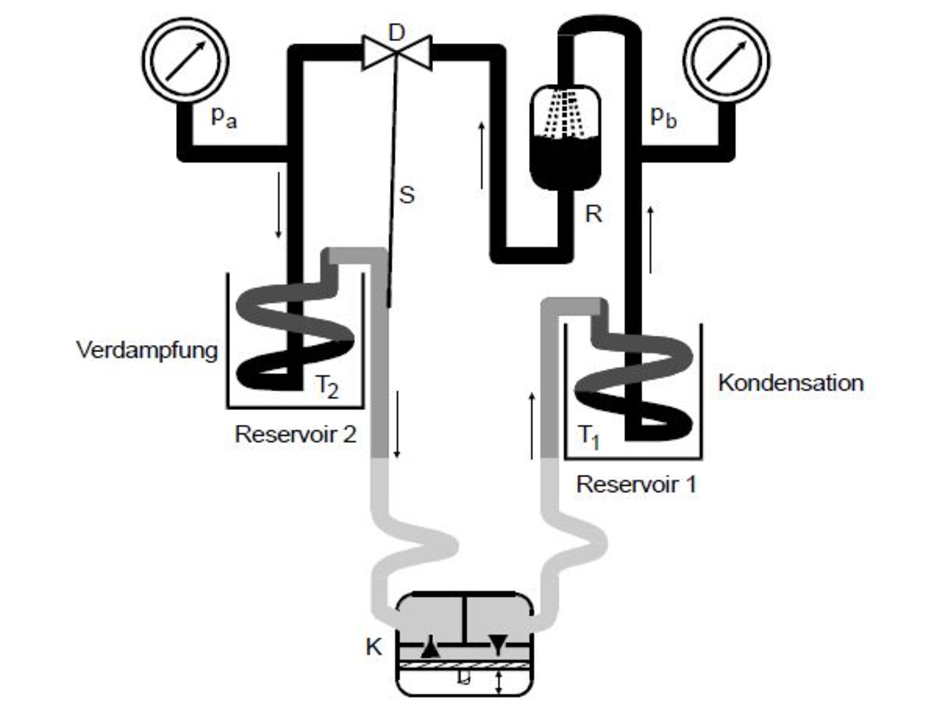
\includegraphics[scale=0.75]{aufbau_1.pdf}
               \caption{Prinzipieller Aufbau einer Wärmepumpe ($p_\text{b}$ > $p_\text{a}$; $T_1$ > $T_2$)}
               \label{fig:prinzW}
        \end{figure}
        Der Kompressor K erzeugt eine annähernd adiabatische Kompression, also eine Kompression ohne Wärmeverluste an die Umgebung. 
        Zusätzlich wird durch diese Kompression ein Mediumskreislauf im System ingang gebracht. Durch das Drosselventil D und dem hohen Strömungswiderstand diesem baut sich ein Druckunterschied
        zwischen vor dem Ventil und dannach auf ($p_\text{b}-p_\text{a}$).

        Die Apparatur ist so konzipiert, dass das Gas Reservoir 2 und 1 durchströmt und jeweils sein Zustand in einem der beiden ändert. Dies bedeutet, dass das Gas sich im Reservoir 2 
        vergasförmigt und in Reservoir 1 durch den erhöhten Druck ($p_\text{b}$) wieder verflüssigt und so seine, durch die Vergasung, aufgenommene Wärme wieder abgibt. Die Messgröße der 
        Verdampfungswärme ist L pro Gramm Substanz.  Somit ist das Reservoir 1 das wärmere und Reservoir 2 das kältere.

        Damit die Apparatur störungsfrei arbeiten kann ist es notwendig weitere Armaturen ins System zu integrieren. Diese haben jedoch keinen direkten Einfluss auf die prinzipielle Wirkungsweise. 
        So benutzt man einen sogennanten "`Reiniger"' R, welches das verflüssigte Transportmedium von Gasblasen reinigt, sodass eine blasenfreie Flüssigkeitszufuhr zum Drosselventil D gewährleistet werden kann.
        Zudem wird eine "`Steuerungsvorrichtung"' S für das Drosselventil benutzt, sodass die Durchlässigkeit der Drosselventils über die Temperaturdifferenz zwischen Eingang und Ausgang ($T_2 - T_1$) 
        des Reservoirs 2 gesteuert werden kann.

    %4
    \newpage
    \section{Durchführung}
    Der Versuchsbau ist folgendermaßen:
    \begin{figure}
               \centering
               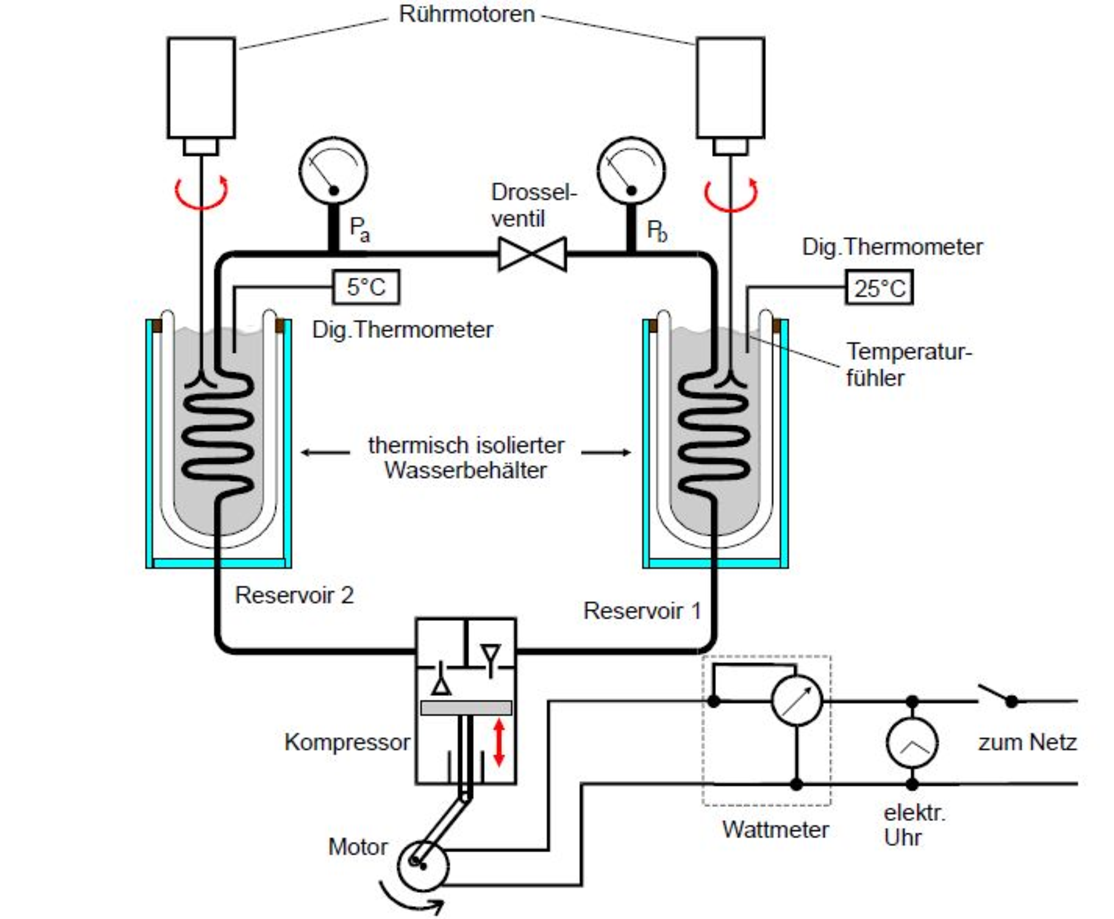
\includegraphics[width=\textwidth]{aufbau_2.pdf}
               \caption{Schematische Darstellung der kompletten Messapparatur}
               \label{fig:scheW}
    \end{figure}

    Sobald der Kompressor eingeschaltet wird, werden die Temperaturen T1 und T2, die Drücke p1 und p2 und die Kompressorleistung N an den Anzeigegeräten abgelesen. Damit die Zeitabstände
    beim Ablesen möglichst gleich sind, werden die Größen immer in derselben Reihenfolge notiert. Um die Drücke p1 und p2 zu erhalten, muss noch 1 bar auf die gemessenen Drücke p*1 und p*2 addiert werden.

    %4
    \newpage
    \section{Messwerte}
    Die folgenden Messwerte wurden uns zur Verfügung gestellt:
    \begin{table}
\centering
\caption{Messdaten}
\label{tab:mess}
\begin{tabular}{
    S[table-format=2.0]
    S[table-format=2.1]
    S[table-format=2.2]
    S[table-format=2.1]
    S[table-format=1.1]
    S[table-format=3.0]
}
\toprule
{$t \mathbin{/} \si{\minute} $} & {$T_1 \mathbin{/} \si{\celsius} $} 
    & {$p_1 \mathbin{/} \si{\bar} $} & {$T_2  \mathbin{/} \si{\celsius} $} 
    & {$p_2 \mathbin{/} \si{\bar} $} & {$N \mathbin{/} \si{\watt} $} \\

\midrule
0  & 21.7 &   4.0   &  21.7 &   4.1  &   120 \\
1  & 23.0 &   5.0   &  21.7 &   3.2  &   120 \\
2  & 24.3 &   5.5   &  21.6 &   3.4  &   120 \\
3  & 25.3 &   6.0   &  21.5 &   3.5  &   120 \\
4  & 26.4 &   6.0   &  20.8 &   3.5  &   120 \\
5  & 27.5 &   6.0   &  20.1 &   3.4  &   120 \\
6  & 28.8 &   6.5   &  19.2 &   3.3  &   120 \\
7  & 29.7 &   6.5   &  18.5 &   3.2  &   120 \\
8  & 30.9 &   7.0   &  17.7 &   3.2  &   120 \\
9  & 31.9 &   7.0   &  16.9 &   3.0  &   120 \\
10 & 32.9 &   7.0   &  16.2 &   3.0  &   120 \\
11 & 33.9 &   7.5   &  15.5 &   2.9  &   120 \\
12 & 34.8 &   7.5   &  14.9 &   2.8  &   120 \\
13 & 35.7 &   8.0   &  14.2 &   2.8  &   120 \\
14 & 36.7 &   8.0   &  13.6 &   2.7  &   120 \\
15 & 37.6 &   8.0   &  13.0 &   2.6  &   120 \\
16 & 38.4 &   8.5   &  12.4 &   2.6  &   120 \\
17 & 39.2 &   8.5   &  11.7 &   2.6  &   120 \\
18 & 40.0 &   9.0   &  11.3 &   2.5  &   120 \\
19 & 40.7 &   9.0   &  10.9 &   2.5  &   120 \\
20 & 41.4 &   9.0   &  10.4 &   2.4  &   120 \\
21 & 42.2 &   9.0   &  9.9  &   2.4  &   120 \\
22 & 42.9 &   9.5   &  9.5  &   2.4  &   120 \\
23 & 43.6 &   9.5   &  9.1  &   2.4  &   120 \\
24 & 44.3 &   10.0  &  8.7  &   2.4  &   120 \\
25 & 44.9 &   10.0  &  8.3  &   2.4  &   120 \\
26 & 45.5 &   10.0  &  8.0  &   2.3  &   120 \\
27 & 46.1 &   10.0  &  7.7  &   2.2  &   122 \\
28 & 46.7 &   10.5  &  7.4  &   2.2  &   122 \\
29 & 47.3 &   10.5  &  7.1  &   2.2  &   122 \\
30 & 47.8 &   10.75 &  6.8  &   2.2  &   122 \\
31 & 48.4 &   11.0  &  5.6  &   2.2  &   122 \\
32 & 48.9 &   11.0  &  4.3  &   2.2  &   122 \\
33 & 49.4 &   11.0  &  3.4  &   2.2  &   122 \\
34 & 49.9 &   11.0  &  3.0  &   2.2  &   122 \\
35 & 50.3 &   11.0  &  2.9  &   2.2  &   122 \\
\bottomrule
\end{tabular}

\end{table}

    %5
    \newpage
    \section{Auswertung}
        \subsection{Aufgabenteil a)}
        \begin{figure}
               \centering
               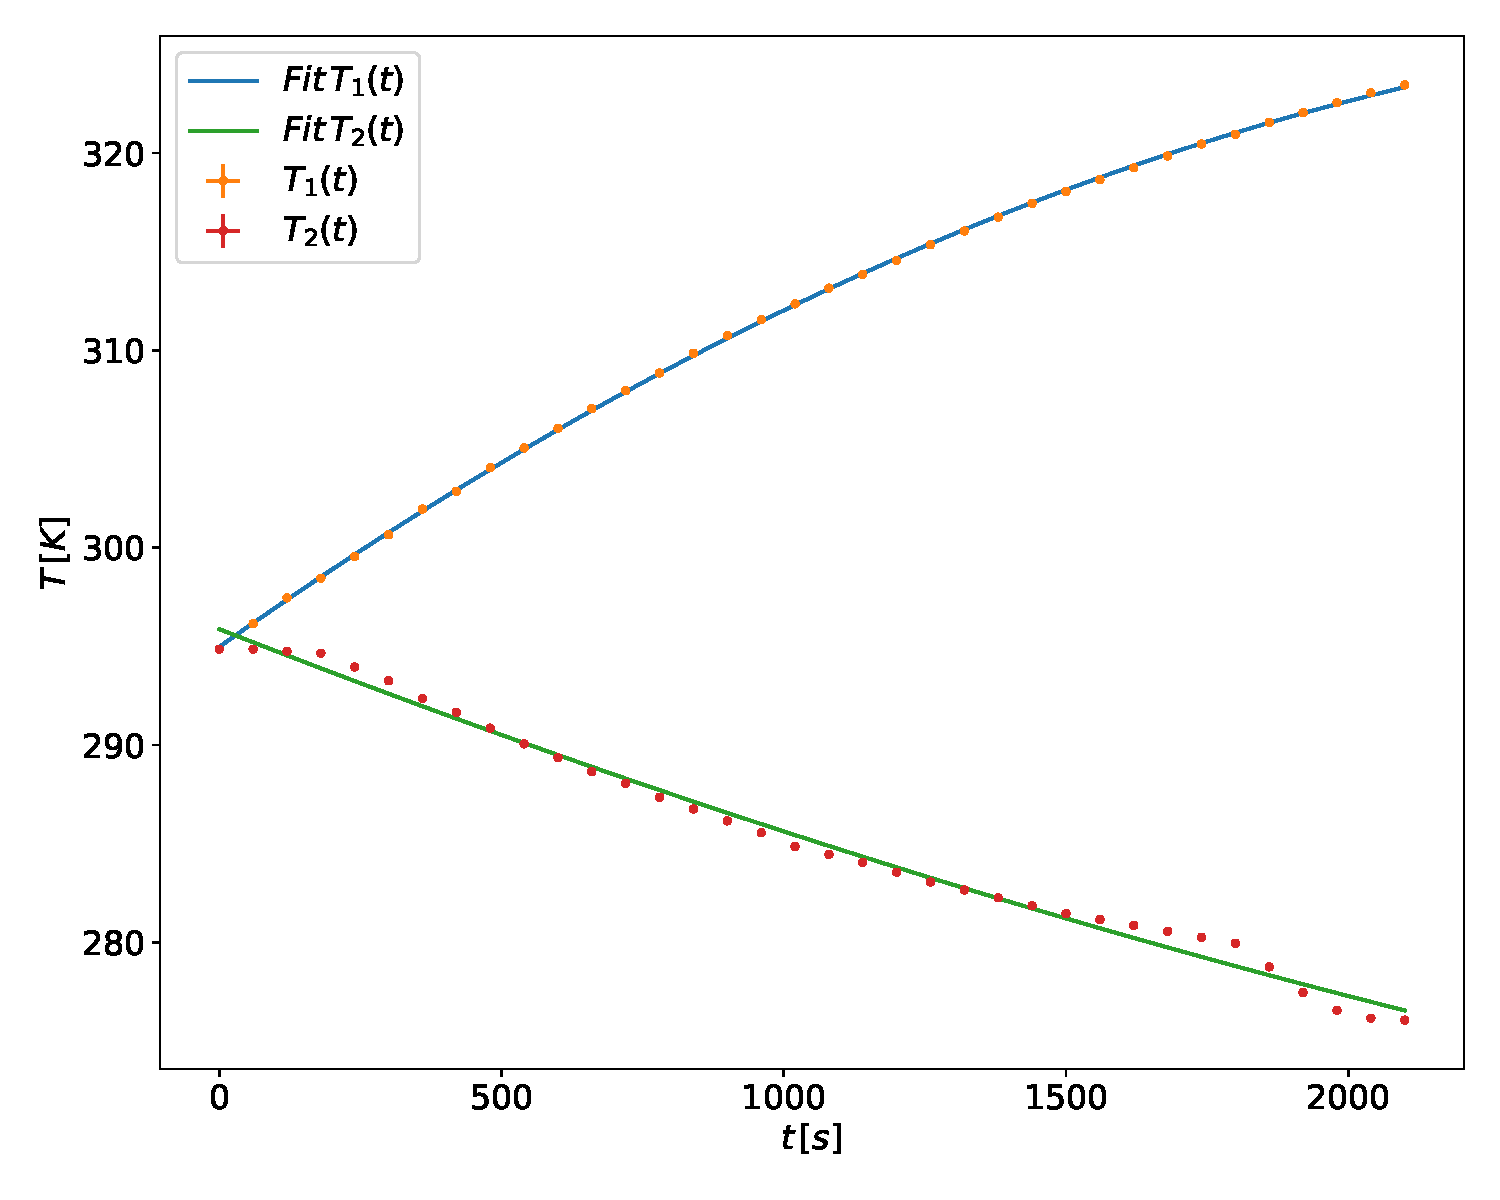
\includegraphics[width=\textwidth]{grafic.pdf}
               \caption{Auswertung mit ausgleichsgeraden}
               \label{fig:grafic}
        \end{figure}


            

        \subsection{Aufgabenteil b)}


        \subsection{Aufgabenteil c)}


        \subsection{Aufgabenteil d)}


        \subsection{Aufgabenteil e)}


        \subsection{Aufgabenteil f)}


        \subsection{Aufgabenteil g)}

    %6
    \section{Literatur}
    %Biber
\end{document}